\chapter
[Rheologic constraints on the upper mantle from five years of
postseismic deformation following the El Mayor-Cucapah earthquake]
{Rheologic constraints on the upper mantle from five years of
postseismic deformation following the El Mayor-Cucapah earthquake\footnote[1]{
This chapter has been published as: Hines, T. T., and Hetland, E. A.
(2016). Rheologic constraints on the upper mantle from five years of
postseismic deformation following the El Mayor-Cucapah earthquake.
Journal of Geophysical Research: Solid Earth, 121,
doi:10.1002/2016JB013114.}}

\section{Abstract}
We analyze five years of Southern California GPS data following the
Mw=7.2 El Mayor-Cucapah earthquake.  We observed transient postseismic
deformation which persists for three years at epicentral distances
greater than ${\sim}200$ km.  In the near-field, rapid postseismic
transience decays to a sustained rate which exceeds its preseismic
trend.  We attempt to determine the mechanisms driving this
deformation, where we consider afterslip at seismogenic depths and
viscoelastic relaxation in the lower crust and upper mantle as
candidate mechanisms.  We find that early, rapid, near-field
deformation can be explained with afterslip on the fault that ruptured
coseismically. The later, sustained, near-field deformation can be
explained with viscoelastic relaxation in the lower crust with a
steady-state viscosity of ${\sim}10^{19}$ Pa s and possibly continued
afterslip.  The postseismic deformation in the far-field is best
explained with a transient viscosity of ${\sim}10^{18}$ Pa s in the
upper mantle. We argue that a transient rheology in the mantle is
preferable over a Maxwell rheology because it better predicts the
decay in postseismic deformation, and also because it does not
conflict with the generally higher, steady-state viscosities inferred
from studies of geophysical processes occurring over longer time
scales.

\section{Introduction}
Ground deformation in the years following a large (Mw$\gtrsim$7)
earthquake can be used to gain insight into the mechanical behavior of
the crust and upper mantle. The interpretations of postseismic
deformation are not always conclusive because multiple postseismic
deformation mechanisms, such as afterslip or viscoelastic relaxation
in the lower crust and upper mantle, can have qualitatively similar
surface expressions \citep[e.g.,][]{Savage1990}. This non-uniqueness
complication can potentially be remedied if the postseismic
deformation occurs in an area that is sufficiently well instrumented
with GPS stations \citep{Hearn2003}.  Owing to the dense geodetic
network deployed throughout the 2000s as part of the Plate Boundary
Observatory, the postseismic deformation following the April 4, 2010,
Mw=7.2 El Mayor-Cucapah earthquake in Baja California was observed at
more GPS stations than any other earthquake in California to date (see
\citet{Hauksson2011} and \citet{Fletcher2014} for a detailed
description of this earthquake and its seismotectonic context).  With
such a large collection of data, we attempt to discern the mechanisms
driving the postseismic deformation. Previous studies which have
modeled postseismic deformation following the El Mayor-Cucapah
earthquake include \citet{Pollitz2012}, \citet{Gonzalez-ortega2014},
\citet{Spinler2015}, and \citet{Rollins2015}. Of these studies,
\citet{Gonzalez-ortega2014} and \citet{Rollins2015} have attempted to
describe the postseismic deformation with afterslip in an elastic
half-space.  \citet{Gonzalez-ortega2014} described five months of
postseismic deformation, observed by InSAR and GPS stations within
${\sim}50$ km of the rupture, with afterslip and contraction on the
coseismically ruptured fault. \citet{Gonzalez-ortega2014} noted that
their preferred model underestimated the GPS displacements for
stations $\gtrsim 25$ km from the rupture and suggested that it could
be the result of unmodeled viscoelastic relaxation.  Using only
continuous GPS stations, which are mostly north of the rupture zone,
\citet{Rollins2015} found that three years of postseismic deformation
can be adequately explained by afterslip, albeit with an implausibly
large amount of slip inferred on the least constrained, southern-most
fault segment. Here, we suggest the afterslip inferred by
\citet{Rollins2015} may have been acting as a proxy for distributed
relaxation in the upper mantle.

\citet{Pollitz2012}, \citet{Rollins2015} and \citet{Spinler2015}
explored viscoelastic relaxation in the lower crust and upper mantle
as a potential postseismic deformation mechanism. The rheology of the
crust and mantle is largely unknown and so modeling postseismic
deformation with viscoelastic relaxation requires one to assume a
rheologic model and then find the best fitting rheologic parameters.
The inference of these rheologic parameters is a computationally
expensive non-linear inverse problem which is typically approached
with a forward modeling grid search method.  Consequently, a
simplified structure for the Earth must be assumed in order to
minimize the number of rheologic parameters that need to be estimated.
For example, it is commonly assumed that the lower crust and upper
mantle are homogeneous, Maxwell viscoelastic layers, which may be too
simplistic for postseismic studies \citep{Riva2009,Hines2013}. To
further reduce the dimensions of the model space, it is also necessary
to make simplifying assumptions about the behavior of afterslip. For
example, one can assume a frictional model for afterslip and
parametrize afterslip in terms of the unknown rheologic properties of
the fault \citep[e.g.,][]{Johnson2009,Johnson2004}. One can also
assume that afterslip does not persist for more than a few months and
then model the later postseismic deformation assuming it to be the
result of only viscoelastic relaxation
\citep[e.g.,][]{Pollitz2012,Spinler2015}. However, afterslip in
similar tectonic settings has been observed to persist for decades
following earthquakes \citep{Cakir2012,Cetin2014}. Indeed, the
preferred viscoelastic model from \citet{Pollitz2012} significantly
underestimates deformation in the Imperial Valley, which could be
indicative of unmodeled continued afterslip.  Neglecting to allow for
sustained afterslip as a postseismic mechanism could then lead to
biased inferences of viscosities.

In this study, we perform a kinematic inversion for fault slip,
allowing it to persist throughout the postseismic period, while
simultaneously estimating the viscosity of the lower crust and upper
mantle.  We create an initial model of the fault slip and effective
viscosity necessary to describe early postseismic deformation using
the method described in \citet{Hines2016}.  This method uses a
first-order approximation of surface deformation resulting from
viscoelastic relaxation which is only applicable to the early
postseismic period. In this case, our initial model describes the
first 0.8 years of postseismic deformation following the El
Mayor-Cucapah earthquake.  We then use the inferred effective
viscosity structure from the initial model to create a suite of
postseismic models which we test against the five years of postseismic
data available to date.  Of the suite of models tested, we find that
postseismic deformation following the El Mayor-Cucapah earthquake can
be explained with a combination of afterslip on a fault segment
running through the Sierra Cucapah and viscoelastic relaxation in a
Zener rheology upper mantle with a transient viscosity on the order of
$10^{18}$ Pa s.

\begin{figure}
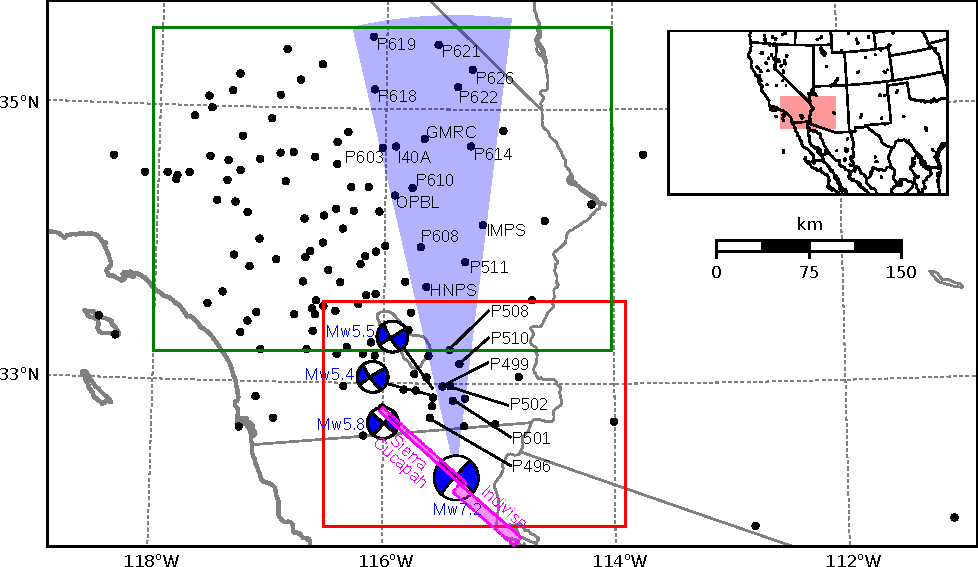
\includegraphics[scale=1.0]{ch3/figures/2016jb013114-p01} 
\caption
[Map of the region considered in this study]
{Map of the region considered in this study.  The large focal
mechanism is the GCMT solution for the El Mayor-Cucapah earthquake,
and the three small focal mechanisms are for the Ocotillo earthquake
and the two main shocks during the Brawley swarm.  The black dots
indicate the locations of GPS stations used in this study.  The fault
geometry used in this study is shown in magenta where dashed lines
indicate buried edges of the fault segments.  The green and red boxes
demarcate the extent of the near-field and far-field maps (Figures
\ref{ch3:fig:NearField} and \ref{ch3:fig:FarField}).  Stations inside
the blue sector, which highlights the area within 10$^\circ$ of the El
Mayor-Cucapah P-axis, are used in Figures
\ref{ch3:fig:RecordSectionMain} and \ref{ch3:fig:RecordSection1}.}
\label{ch3:fig:ContextMap}
\end{figure}

\section{Data processing}\label{ch3:sec:Data}
We use continuous GPS position time series provided by University
Navstar Consortium (UNAVCO) for stations within a 400 km radius about
the El Mayor-Cucapah epicenter. We collectively describe the coseismic
and postseismic displacements resulting from the El Mayor-Cucapah
earthquake as $u_\mathrm{post}(t)$.  We consider the GPS position time
series, $u_\mathrm{obs}(t)$, to be the combination of
$u_\mathrm{post}(t)$, secular tectonic deformation, annual and
semi-annual oscillations, and coseismic offsets from significant
earthquakes over the time span of this study.  The June 14, 2010,
Mw=5.8 Ocotillo earthquake and the Brawley swarm, which included an
Mw=5.5 and an Mw=5.4 event on August 26, 2012 (Figure
\ref{ch3:fig:ContextMap}), are the only earthquakes that produced
noticeable displacements in any of the time series.  We treat the
displacements resulting from the Brawley swarm as a single event
because the daily solutions provided by UNAVCO cannot resolve the
separate events.  Although the Ocotillo earthquake had its own series
of aftershocks \citep{Hauksson2011}, neither the Ocotillo earthquake
nor the Brawley swarm produced detectable postseismic deformation.  We
model displacements resulting from these events with only a Heaviside
function, $H(t)$, describing the coseismic offsets.  We then model
$u_\mathrm{obs}(t)$ as
\begin{equation}
  u_\mathrm{obs}(t) = u_\mathrm{pred}(t) + \epsilon,
\end{equation}
where
\begin{equation}\label{TimeSeriesModel}
  \begin{split}  
    u_\mathrm{pred}(t) = &u_\mathrm{post}(t)H(t-t_\mathrm{emc}) + c_0 + c_1t + \\
                         &c_2\sin(2\pi t) + c_3\cos(2\pi t) + c_4\sin(4\pi t) + c_5\cos(4\pi t) + \\
                         &c_6H(t-t_\mathrm{oc}) + c_7H(t-t_\mathrm{bs}).
  \end{split}
\end{equation}
In the above equations, $t_\mathrm{emc}$, $t_\mathrm{oc}$ and
$t_\mathrm{bs}$ are the times of the El Mayor-Cucapah earthquake,
Ocotillo earthquake, and the Brawley swarm, respectively, $c_0$
through $c_7$ are unknown coefficients, and $\epsilon$ is the
observation noise.  We are using years as our unit of time which makes
$c_2$ through $c_5$ the coefficients for annual and semi-annual
oscillations.  We only estimate jumps associated with the Ocotillo
earthquake and Brawley swarm for stations within 40 km of their
epicenters.

Stations which recorded displacements that clearly cannot be described
by the aforementioned processes are not included in our analysis. This
includes stations in the Los Angeles basin, where anthropogenic
deformation can be larger than the postseismic signal that we are
trying to estimate \citep{Bawden2001,Argus2005}. In order to ensure an
accurate estimation of the secular deformation, we only use stations
that were installed at least six months prior to El Mayor-Cucapah
earthquake even though several GPS stations were installed after the
earthquake to get better coverage of the postseismic deformation field
\citep{Spinler2015}.  It would be possible to subtract secular
velocities derived from elastic block models
\citep[e.g.,][]{Meade2005} from velocities recorded at the newly
installed stations to get an estimate of postseismic velocities at
those stations. However, estimating velocities from an already noisy
displacement time series can introduce significant uncertainties
depending on exactly how the estimation is done.  We therefore use
coseismic and postseismic displacements, rather than velocities, in
our inverse method described in Section \ref{ch3:sec:Model}. This
choice prevents us from using the newly installed stations for our
analysis.

The October 16, 1999, Mw=7.1 Hector Mine earthquake, which occurred
${\sim}270$ km north of the El Mayor-Cucapah epicenter, produced
transient postseismic deformation which we do not wish to model,
either mechanically or through empirical line fitting.  We thus
restrict our analysis to deformation observed six years after the
Hector Mine earthquake, which is when postseismic velocities at sites
near the Hector Mine epicenter are approximately constant
\citep{Savage2009}. When appraising our model fit in Section
\ref{ch3:sec:Model}, we see some systematic residuals in the vicinity
of the Hector Mine epicenter, which may be the result of errors in the
assumption that the trend in Hector Mine postseismic deformation is
linear after six years.

Studies of postseismic deformation typically assume a parametric form
for $u_\mathrm{post}(t)$, such as one with a logarithmic or
exponential time dependence \citep[e.g.,][]{Savage2005a}.  However, by
assuming a logarithmic or exponential form of $u_\mathrm{post}(t)$ we
run the risk of over fitting the GPS time series and inferring a
non-existent postseismic signal. We therefore do not assume any
parametric form for $u_\mathrm{post}(t)$ and rather treat it as
integrated Brownian motion, so that
\begin{equation}
    \dot{u}_\mathrm{post}(t) = \sigma^2\int_0^t w(s) ds,
\end{equation}    
where $w(t)$ is white noise and the variance of
$\dot{u}_\mathrm{post}(t)$ increases linearly with time by a factor of
$\sigma^2$. We use a Kalman filtering approach to estimate
$u_\mathrm{post}(t)$ and the unknown parameters in eq.
(\ref{TimeSeriesModel}).  In the context of Kalman filtering, our time
varying state vector is
\begin{equation}
    \mathbf{X}(t) = [u_\mathrm{post}(t),\dot u_\mathrm{post}(t), c_0, ..., c_7]
\end{equation}
and eq. (\ref{TimeSeriesModel}) is the observation function which maps
the state vector to the GPS observations. We initiate the Kalman
filter by assuming a prior estimate of $\mathbf{X}(t)$ at the first
time epoch, denoted $\mathbf{X}_{1|0}$, which has a sufficiently large
covariance, denoted $\mathbf{\Sigma}_{1|0}$, to effectively make our
prior uninformed.  For each time epoch, $t_i$, Bayesian linear
regression is used to incorporate GPS derived estimates of
displacement with our prior estimate of the state,
$\mathbf{X}_{i|i-1}$, to form a posterior estimate of the state,
$\mathbf{X}_{i|i}$, which has covariance $\mathbf{\Sigma}_{i|i}$.  We
then use the posterior estimate of the state at time $t_i$ to form a
prior estimate of the state at time $t_{i+1}$ through the transition
function
\begin{equation}\label{predict}
  \mathbf{X}_{i+1|i} = \mathbf{F}_{i+1}\mathbf{X}_{i|i} + \mathbf{\delta}_{i+1}, 
\end{equation}
where 
\begin{equation}
  \mathbf{F}_{i+1} = 
  \left[
  \begin{array}{ccc}
    1           & (t_{i+1} - t_i) & \mathbf{0}\\
    0           & 1              & \mathbf{0}\\
    \mathbf{0}  & \mathbf{0}     & \mathbf{I}
  \end{array}
  \right]
\end{equation}
and $\mathbf{\delta}_{i+1}$ is the process noise, which has zero mean
and covariance described by
\begin{equation}
  \mathbf{Q}_{i+1} = 
  \sigma^2 \left[
  \begin{array}{ccc}
  \frac{(t_{i+1} - t_i)^3}{3} & \frac{(t_{i+1} - t_{i})^2}{2} & \mathbf{0}\\
  \frac{(t_{i+1} - t_i)^2}{2} & (t_{i+1} - t_{i}) & \mathbf{0}\\ 
  \mathbf{0} & \mathbf{0} & \mathbf{0}
  \end{array}
  \right].
\end{equation}
The covariance of the new prior state, $\mathbf{X}_{i+1|i}$, is then
described by
\begin{equation}
  \mathbf{\Sigma}_{i+1|i} = \mathbf{F}_{i+1}\mathbf{\Sigma}_{i|i}\mathbf{F}^T_{i+1} + \mathbf{Q}_{i+1}.
\end{equation}
This process is repeated for each of the $N$ time epochs.  We then use
Rauch-Tung-Striebel smoothing \citep{Rauch1965} to find
$\mathbf{X}_{i|N}$, which is an estimate of the state at time $t_i$
that incorporates GPS observation for all $N$ time epochs.  Our final
estimates of $u_\mathrm{post}(t)$ are used in subsequent analysis,
while the remaining components of the state vector are considered
nuisance parameters. In the interests of computational tractability,
we down sample our smoothed time series from daily solutions down to
weekly solutions.

The smoothness of $u_\mathrm{post}(t)$ is controlled by the chosen
value of $\sigma$, which describes how rapidly we expect postseismic
displacements to vary over time.  Setting $\sigma$ equal to zero will
effectively result in modeling $u_\mathrm{post}(t)$ as a straight line
which is insufficient to describe the expected transient behavior in
postseismic deformation. The other end member, where $\sigma$ is
infinitely large, will result in $u_\mathrm{pred}(t)$ overfitting the
data. While one can use a maximum likelihood based approach for
picking $\sigma$ \citep[e.g.,][]{Segall1997}, we instead take a
subjective approach and choose a value for $\sigma$ that is just large
enough to faithfully describe the observed deformation at the most
near-field station in our study, P496, which exhibits the most rapid
changes in velocity. This ensures that $\sigma$ will be sufficiently
large so that our estimate of $u_\mathrm{post}(t)$ does not smooth out
potentially valuable postseismic signal at the remaining stations. We
find that using $\sigma = 50\ \mathrm{mm}/\mathrm{yr}^{1.5}$
adequately describe all but the first week of postseismic deformation
at station P496, which slightly increases our estimate of coseismic
displacements (Figure \ref{ch3:fig:P496}).  We include an example of
estimating $u_\mathrm{post}(t)$ for a far-field station, P619, which
is about 359 km north of the El Mayor-Cucapah epicenter (Figure
\ref{ch3:fig:P619}).  At station P619, along with all the other
stations in the Mojave region, there is a south-trending postseismic
transience that persists for the first three years after the El
Mayor-Cucapah earthquake.  Postseismic deformation that extends to
these epicentral distances has also been observed after the Hector
Mine earthquake \citep{Freed2007a}.

\begin{figure}
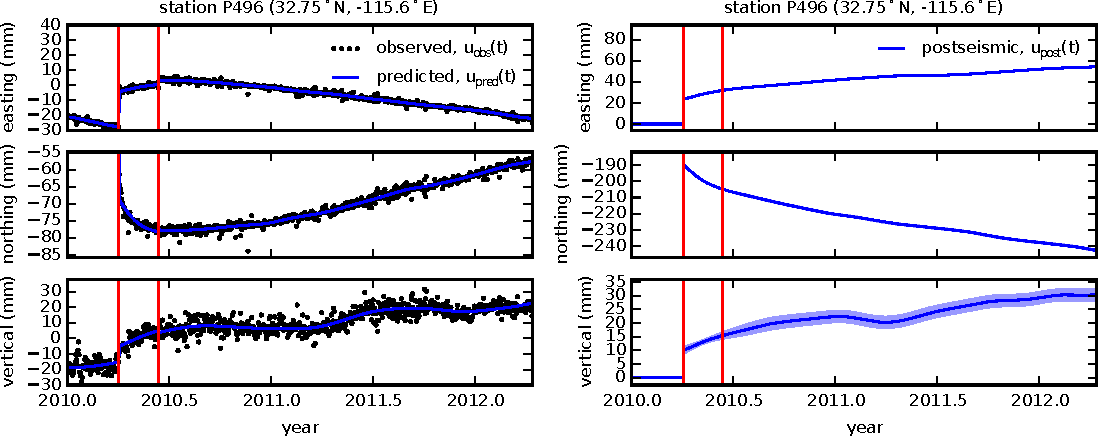
\includegraphics[scale=0.9]{ch3/figures/2016jb013114-p02}
\caption
[Observed displacements and estimated postseismic displacements
for station P496] 
{Left panels show GPS time series from UNAVCO (black) and the
predicted displacement (blue) from eq. (\ref{TimeSeriesModel}) for a
near-field station.  Red lines indicate the times of the El
Mayor-Cucapah and Ocotillo earthquake. The right panels show estimated
coseismic and postseismic displacements, $u_\mathrm{post}$, which are
extracted from the predicted displacements.  The 68\% confidence
interval is shown in light blue.}
\label{ch3:fig:P496}
\end{figure}

\begin{figure}
\noindent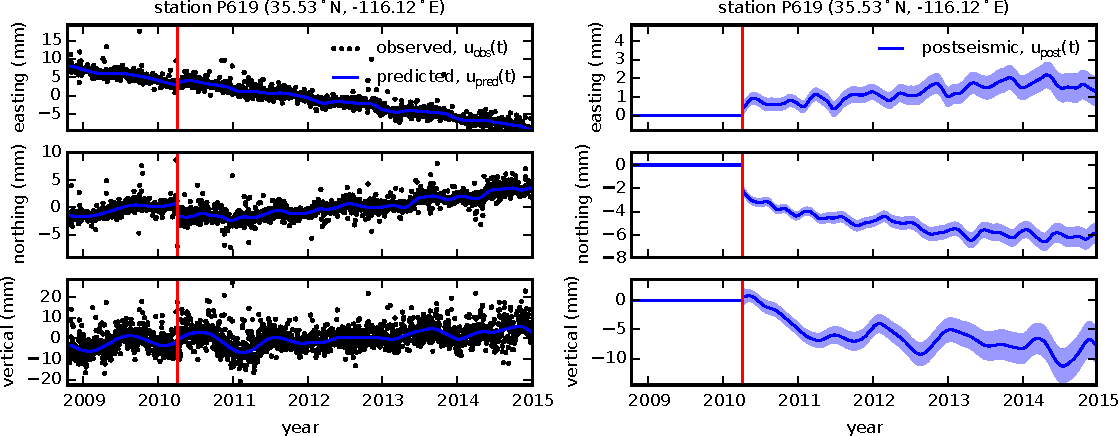
\includegraphics[scale=0.9]{ch3/figures/2016jb013114-p03}
\caption
[Observed displacements and estimated postseismic displacements
for station P619] 
{same as Figure \ref{ch3:fig:P496} but for a far-field station.} 
\label{ch3:fig:P619}
\end{figure}

It is important to note that the shown uncertainties in
$u_\mathrm{post}(t)$ do not account for the non-negligible epistemic
uncertainty in eq. (\ref{TimeSeriesModel}).  For example, we assume a
constant rate of secular deformation, which appears to be an
appropriate approximation for all but perhaps the stations closest to
the Hector Mine epicenter, as noted above.  Also, our model for
seasonal deformation in eq. (\ref{TimeSeriesModel}) assumes a constant
amplitude over time, which means that any yearly variability in the
climatic conditions could introduce systematic residuals
\citep{Davis2012}. Indeed, it would be more appropriate to consider
the seasonal amplitudes $c_2-c_5$ in eq. (\ref{TimeSeriesModel}) as
stochastic variables \citep{Murray2005}. By using constant seasonal
amplitudes, our estimate of $u_\mathrm{post}(t)$ seems to describe
some of the unmodeled annual and semi-annual oscillations (e.g. Figure
\ref{ch3:fig:P619}).

We show in Figures \ref{ch3:fig:NearField} and \ref{ch3:fig:FarField}
the near and far-field coseismic displacements and the postseismic
displacements accumulated over the time intervals 0-1 years, 1-3
years, and 3-5 years.  Stations at epicentral distances beyond
${\sim}200$ km have an elevated rate of deformation for the first
three years following the earthquake.  This far-field deformation is
trending southward at a rate of a few millimeters per year along the
direction of the El Mayor-Cucapah P-axis.  A similar eastward trend
can be seen in the few far-field stations in Arizona, located along
the T-axis.  After three years, the trend in far-field postseismic
deformation is barely perceptible.  Most far-field stations display an
initial subsidence for the first year after the El Mayor-Cucapah
earthquake followed by continued uplift.  This trend in vertical
deformation can be observed in all three of the quadrants where
postseismic data is available, which means that the vertical
deformation does not exhibit an anti-symmetric quadrant pattern, as
would be expected for postseismic processes.  Although we use vertical
deformation in our analysis in Section \ref{ch3:sec:Model}, we do not
put an emphasis on trying to describe the vertical deformation because
it likely does not have postseismic origins.

\begin{figure}
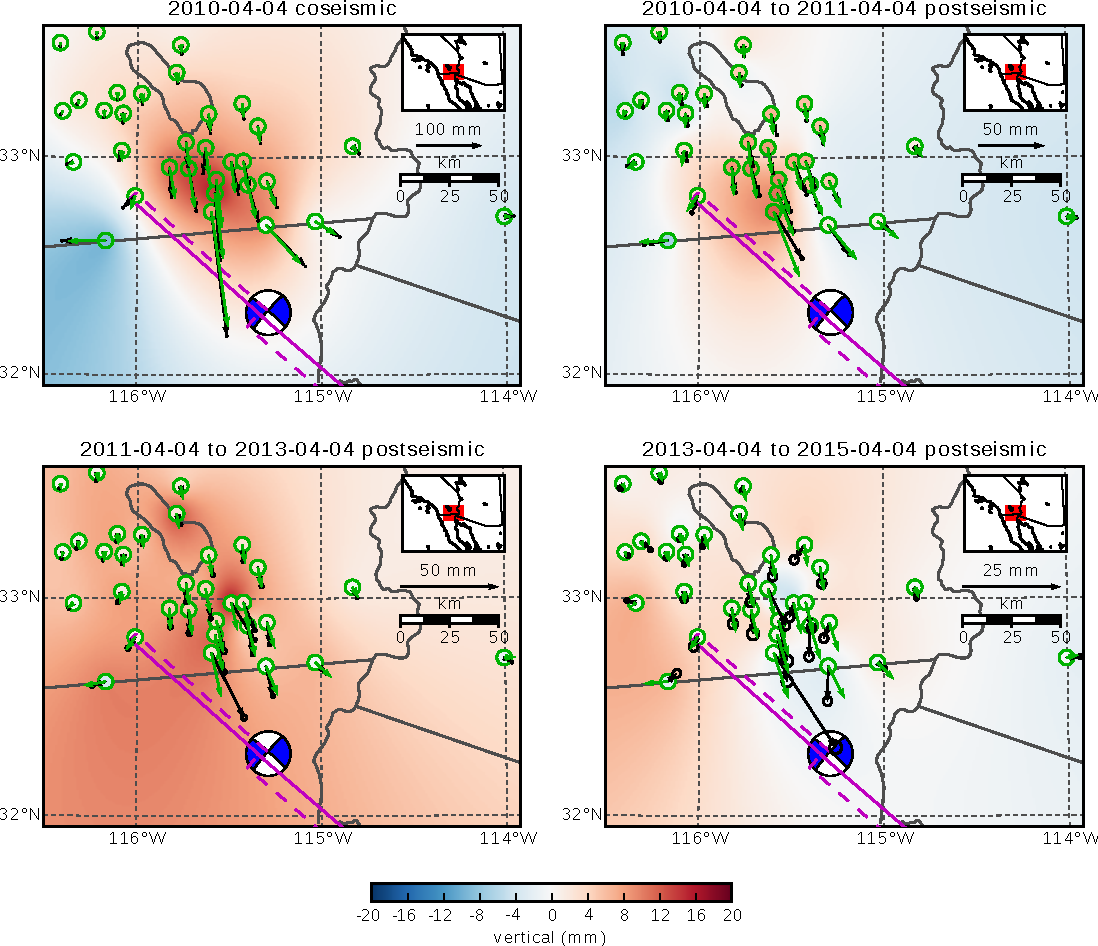
\includegraphics[scale=0.9]{ch3/figures/2016jb013114-p04}
\caption
[Observed and predicted near-field postseismic deformation]
{Near-field coseismic and cumulative postseismic displacements
over the indicated time periods (black) and predicted displacements
for our preferred model from Section \ref{ch3:sec:FullInversion}
(green).  The black error ellipses show the 68\% confidence interval
for the observed horizontal displacements.  Observed vertical
displacements are shown as an interpolated field and predicted
vertical displacements are shown within the green circles.  Note that
the interpolant is not well constrained in Mexico where there is no
data available.}
\label{ch3:fig:NearField}
\end{figure}

\begin{figure}
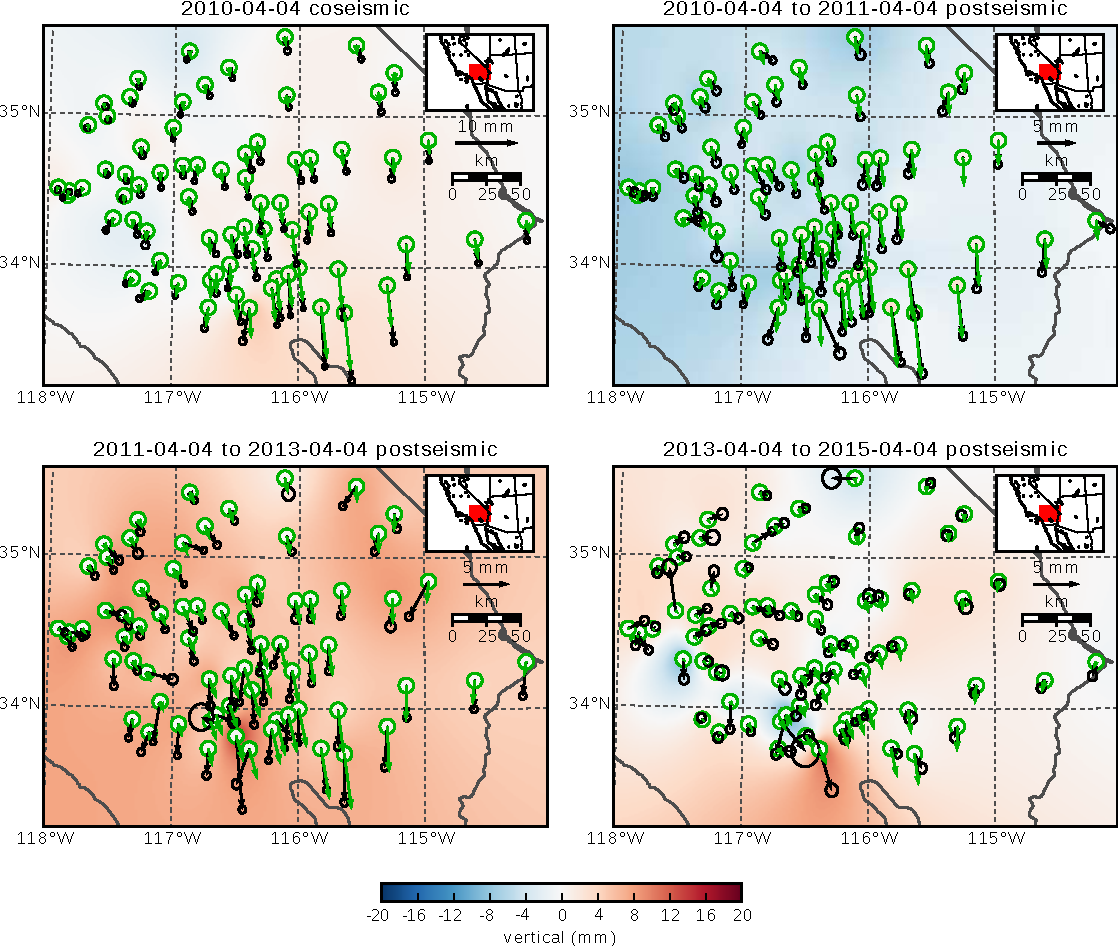
\includegraphics[scale=0.9]{ch3/figures/2016jb013114-p05}
\caption
[Observed and predicted far-field postseismic deformation]
{Same as Figure \ref{ch3:fig:NearField} but for far-field stations.}
\label{ch3:fig:FarField}
\end{figure}

The near-field postseismic deformation is notably sustained when
compared to the far-field deformation.  Namely, the station in this
study which is closest to the El Mayor-Cucapah epicenter, P496, has a
steady postseismic trend of ${\sim}1.5$ cm/yr to the south after about
one year.  Vertical postseismic deformation in the near-field does
display a quadrant pattern which is consistent with the coseismic
vertical deformation, suggesting that it is resulting from postseismic
processes.  However, the vertical postseismic signal is only apparent
for the first year after the earthquake (Figure
\ref{ch3:fig:NearField}).  As with the far-field deformation, there is
a general trend of uplift in the near-field after about one year.

\section{Postseismic modeling}\label{ch3:sec:Model}

\begin{table}\label{ch3:tab:MaterialProperties}
\begin{tabular} {l l l l l}
depth (km) &$\lambda$ (GPa)&$\mu$ (GPa)&$\eta_\mathrm{eff}$ ($10^{18}$ Pa s) & $\mu_\mathrm{k}/\mu$\\ \hline
0-5 & 24.0 & 24.0 & - & -\\
5-15 & 35.0 & 35.0 & - & -\\
15-30 & 42.0 & 42.0 & 44.3 & 0.0\\
30-60 & 61.0 & 61.0 & 5.91 & 0.375\\
60-90 & 61.0 & 61.0 & 1.99 & 0.375\\
90-120 & 61.0 & 61.0 & 1.31 & 0.375\\
120-150 & 61.0 & 61.0 & 1.10 & 0.375\\
150-$\infty$ & 61.0 & 61.0 & 1.07 & 0.375\\
\end{tabular}
\caption
[Assumed and estimated material properties]
{Assumed and estimated material properties. $\lambda$ and
$\mu$ are assumed known \textit{a priori} and are based on the values
used for the coseismic model by \citet{Wei2011}.  The values for
$\eta_\mathrm{eff}$ are estimated in Section
\ref{ch3:sec:InitialInversion}, and $\frac{\mu_k}{\mu}$ are the
optimal shear moduli ratios found in Section
\ref{ch3:sec:FullInversion} for a Zener rheology upper mantle.}
\end{table}

We seek to find the mechanisms driving five years of postseismic
deformation following the El Mayor-Cucapah earthquake and we consider
afterslip and viscoelastic relaxation as candidate mechanisms.
Poroelastic rebound has also been used to model postseismic
deformation \citep[e.g.,][]{Jonsson2003}; however,
\citet{Gonzalez-ortega2014} found that poroelastic rebound is unlikely
to be a significant contributor to postseismic deformation following
the El Mayor-Cucapah earthquake. Furthermore, we consider stations
which are sufficiently far away from the rupture that poroelastic
rebound should be insignificant.

We estimate coseismic and time-dependent postseismic fault slip, both
of which are assumed to occur on a fault geometry modified from
\citet{Wei2011}.  Field studies \citep{Fletcher2014} and LIDAR
observations \citep{Oskin2012} have revealed a significantly more
complicated fault geometry than what was inferred by \citet{Wei2011},
especially within the Sierra Cucapah.  However, we find that a
relatively simple coseismic fault geometry based on \citep{Wei2011} is
adequate because most of the stations used in this study are
sufficiently far from the El Mayor-Cucapah rupture that they are
insensitive to the details in the fault geometry found by
\citet{Fletcher2014} and \citet{Oskin2012}.  The fault geometry used
in this study (Figure \ref{ch3:fig:ContextMap}) consists of the two
main fault segments inferred by \citet{Wei2011}, where the northern
segment runs through the Sierra Cucapah up to the US-Mexico border and
the southern segment is the Indiviso fault which extends down to the
Gulf of California. Both segments extend from the surface to 15 km
depth.  We extend the northern segment by 40 km to the northwest,
which is motivated by the clustering of aftershocks on the northern
tip of the coseismic rupture zone \citep{Hauksson2011,Kroll2013}.
This extended fault segment was also found to be necessary by
\citet{Rollins2015} and \citet{Pollitz2012} in order to describe the
postseismic deformation.

\subsection{Elastic postseismic inversion}\label{ch3:sec:ElasticInversion}    
We consider a variety of rheologic models for the lower crust and
upper mantle. The simplest rheologic model is to consider them to be
effectively elastic and isotropic.  In such case, the rheologic
parameters consist of the reasonably well known Lam\'e parameters,
$\lambda$ and $\mu$, and we use the same values used by
\citet{Wei2011} throughout this paper (Table 4.1).  The only unknown is
the distribution of fault slip, which can be estimated from
postseismic deformation through linear least squares.
\citet{Rollins2015} used a subset of the GPS stations considered in
this study and found that three years of postseismic deformation
following the El Mayor-Cucapah earthquake can be explained with
afterslip on the coseismic fault plane without requiring any
viscoelastic relaxation. We also perform an elastic slip inversion,
but we use GPS stations within a larger radius about the El
Mayor-Cucapah epicenter (400 km instead of ${\sim}200$ km). Our
forward problem describing predicted postseismic deformation,
$u_\mathrm{pred}$, in terms of time dependent fault slip, $s$, is
\begin{equation}\label{ch3:eq:ElasticForward}
  u_\mathrm{pred}(x,t) = \int_F s(\xi,t)g(x,\xi)d\xi, 
\end{equation}           
where $F$ denotes the fault and $g(x,\xi)$ is the elastic Green's
function describing displacement at surface position $x$ resulting
from slip at $\xi$ on the fault.  We estimate coseismic slip and the
rate of afterslip over the postseismic time intervals 0.0-0.125,
0.125-0.25, 0.25-0.5, 0.5-1.0, 1.0-2.0, 2.0-3.0, 3.0-4.0, and 4.0-5.0
years.  Each fault segment is discretized into roughly 4 km by 4 km
patches an we impose that the direction of slip and slip rate are
within 45$^\circ$ of right-lateral. We also add zeroth-order Tikhonov
regularization so that our solution for $s$ satisfies
\begin{equation}\label{ch3:eq:ElasticObjective}
  \min_s \left(\left|\left|\frac{u_\mathrm{pred}(s) - u_\mathrm{post}}                
                                {\sigma_\mathrm{post}}\right|\right|_2^2 + 
                                \lambda_s||s||_2^2\right),
\end{equation}
where $\sigma_\mathrm{post}$ is the uncertainty on postseismic
displacements and $\lambda_s$ is a penalty parameter which is chosen
with a trade-off curve.  We use Pylith \citep{Aagaard2013} to compute
the Green's functions for this inversion as well as for the remaining
inversions in this paper.

Our coseismic slip and afterslip solutions are shown in Figure
\ref{ch3:fig:ElasticSlip}.  Similar to \citet{Rollins2015}, we find
that a large amount of afterslip on the Indiviso fault segment is
required to explain the observations. The potency of our inferred
coseismic slip is $3.2\times10^9\ \mathrm{m}^3$, equivalent to a
Mw=7.28 earthquake when assuming a shear modulus of 32 GPa.  The
potency of our inferred cumulative five years of afterslip is
$6.1\times10^9\ \mathrm{m}^3$, equivalent to a Mw=7.46 earthquake,
which is unrealistically large if we consider afterslip to be driven
by coseismically induced stresses.  Figure
\ref{ch3:fig:RecordSectionMain} shows the time series for the observed
and predicted postseismic displacements at stations along the El
Mayor-Cucapah P-axis.  We show the radial component of displacements
with respect to the El Mayor-Cucapah epicenter and we also rescale the
displacements so that the difference between the minimum and maximum
observed displacements are the same for each station.  Our elastic
slip model accurately describes near-field postseismic deformation and
systematically underestimates postseismic deformation at epicentral
distances ${\gtrsim}150$ km.  When the fault segments used in the
inversion are extended down to 30 km depth, rather than 15 km, the
systematic far-field residuals are smaller but remain apparent.
Because an elastic model requires an unrealistic amount of afterslip
and is unable to predict far-field deformation, we move on to consider
viscoelastic models in the next section.

\begin{figure}
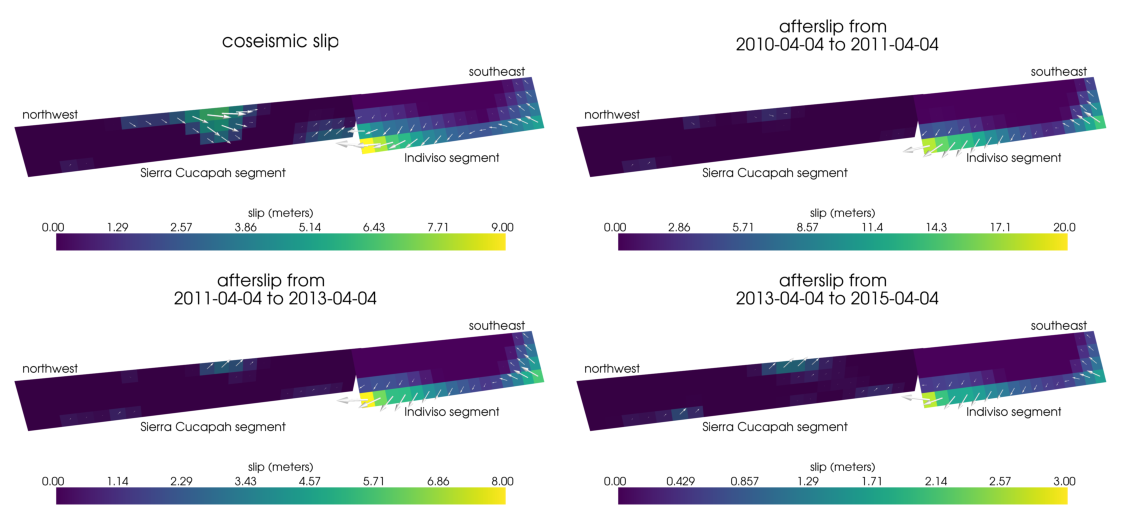
\includegraphics[scale=0.9]{ch3/figures/2016jb013114-p06}
\caption
[Inferred coseismic slip and afterslip when assuming an elastic
lithosphere]
{Coseismic slip and cumulative afterslip over the indicated
time intervals when assuming the crust and mantle are elastic.  Color
indicates the magnitude of slip and arrows indicate the motion of the
hanging wall.}
\label{ch3:fig:ElasticSlip}
\end{figure}

\begin{figure}
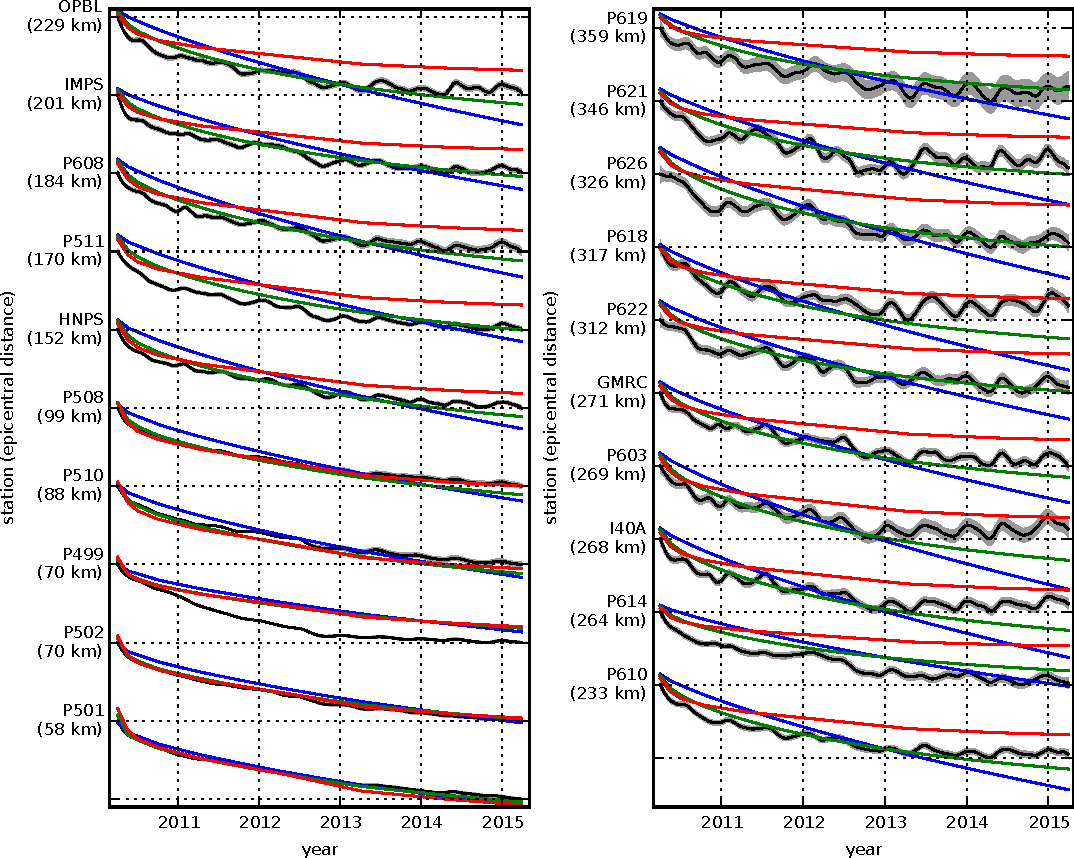
\includegraphics[scale=0.9]{ch3/figures/2016jb013114-p07}
\caption
[Radial components of observed and predicted postseismic displacments]
{Scaled radial component of postseismic displacements.
Downward motion indicates that the station is moving toward the El
Mayor-Cucapah epicenter.  Displacement time series are scaled so that
the minimum and maximum observed values lie on the grid lines.  The
observed postseismic displacements, $u_\mathrm{post}$ are shown in
black with gray indicating the 68\% confidence interval.  The
displacements predicted by the best fitting elastic model are shown in
red.  The blue and green lines are the predicted postseismic
displacements for the models discussed in Section
\ref{ch3:sec:FullInversion}. The blue lines show the predicted
displacements for the model with a Maxwell viscoelastic lower crust
and upper mantle.  The green line shows the predicted displacements
for our preferred model, which has a Maxwell viscoelastic lower crust
and a Zener viscoelastic upper mantle.  The effective viscosities are
the same for both models and are shown in Figure
\ref{ch3:fig:EffectiveViscosity}.}
\label{ch3:fig:RecordSectionMain}
\end{figure}

\subsection{Early postseismic inversion}\label{ch3:sec:InitialInversion}
For any linear viscoelastic rheology of the crust and mantle,
postseismic displacements resulting from time dependent fault slip can
be described as
\begin{equation}\label{GeneralForward}
  u_\mathrm{pred}(x,t) = \int_F s(\xi,t)g(x,\xi)d\xi + 
           \int_0^t\int_F s(\xi,\tau) f(t-\tau,x,\xi) d\xi d\tau,
\end{equation}
where $f(t,x,\xi)$ describes the time-dependent velocity at $x$
resulting from viscoelastic relaxation of stresses induced by slip at
$\xi$. $f$ is a function of $\lambda$, $\mu$, and any additional
rheologic parameters controlling the viscoelastic response, which are
generally not well known. Schematic representations of the
viscoelastic rheologic models considered in this study are shown in
Figure \ref{ch3:fig:Rheology}.  We discuss these rheologic models and
their use in geophysical studies in Section \ref{Discussion}.

\begin{figure}
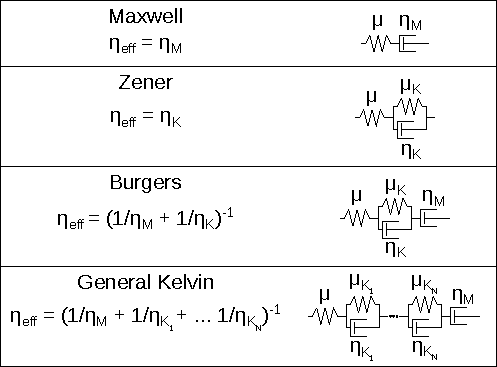
\includegraphics[scale=1.0]{ch3/figures/2016jb013114-f08}
\caption
[Schematic illustration of rheologic models]
{Schematic illustration of the rheologic models considered in
this paper as well as their effective viscosities.}
\label{ch3:fig:Rheology}
\end{figure}

In order to greatly simplify the inverse problem, we use the method
described in \citet{Hines2016} to constrain an initial effective
viscosity structure from the early postseismic deformation.  Our
method uses the fact that coseismic stresses throughout the crust and
upper mantle depend on the instantaneous elastic parameters and are
independent of the viscoelastic parameters which we wish to estimate.
Immediately following an earthquake, each parcel will have a strain
rate that is proportional to the coseismic stress and inversely
proportional to the parcel's effective viscosity, $\eta_\mathrm{eff}$.
Using one-dimensional rheologic models, we define the effective
viscosity as
\begin{equation}
  \eta_\mathrm{eff} = \left.\frac{\sigma}{\dot{\varepsilon}}\right|_{t=0},
\end{equation}
where $\sigma$ is an applied stress at $t=0$ and $\dot\varepsilon$ is
the resulting strain rate.  Figure \ref{ch3:fig:Rheology} shows how
$\eta_\mathrm{eff}$ relates to the parameters for various linear
viscoelastic rheologies.  We can deduce that the initial rate of
surface deformation resulting from viscoelastic relaxation is a
summation of the surface deformation resulting from relaxation in each
parcel, scaled by the reciprocal of the parcel's effective viscosity.
That is to say
\begin{equation}\label{InitialRate}
  f(0,x,\xi) = \int_L \frac{h(x,\xi,\zeta)}{\eta_\mathrm{eff}(\zeta)} d\zeta, 
\end{equation}
where $L$ denotes the crust and mantle and $h(x,\xi,\zeta)$ describes
the initial rate of deformation resulting from viscoelastic relaxation
at $\zeta$ induced by slip at $\xi$. We can combine eq.
(\ref{InitialRate}) with eq. (\ref{GeneralForward}) to get a
first-order approximation for early postseismic deformation,
\begin{equation}\label{ApproxForward}
  u_\mathrm{pred}(x,t) \approx \int_F s(\xi,t)g(x,\xi)d\xi + 
           \int_0^t\int_F\int_L \frac{s(\tau,\xi)}{\eta_\mathrm{eff}(\zeta)} h(x,\xi,\zeta) d\zeta d\xi d\tau,
\end{equation}
which is valid for as long as the rate of deformation resulting from
viscoelastic relaxation is approximately constant.  Although eq.
(\ref{ApproxForward}) may only be valid for a short portion of the
postseismic period, its utility becomes apparent when noting that $g$
and $h$ are only functions of the fault geometry and instantaneous
elastic properties, $\lambda$ and $\mu$, and thus $g$ and $h$ can be
computed numerically as a preprocessing step.  The forward problem in
eq. (\ref{ApproxForward}) can then be rapidly evaluated for any
realization of $s$ and $\eta_{\mathrm{eff}}$.  This is in contrast to
evaluating the full forward problem, eq. (\ref{GeneralForward}),
numerically for each realization of $s$ and the unknown rheologic
properties.

Details on how eq. (\ref{ApproxForward}) is used to estimate $s$ and
$\eta_\mathrm{eff}$ from postseismic deformation can be found in
\citet{Hines2016}.  A non-linear Kalman filter based inverse method
can also be used to estimate $s$ and $\eta_{\mathrm{eff}}$ in a manner
similar to \citet{Segall1997} or \citet{McGuire2003}, in which we
would not have to explicitly impose a time dependent parametrization
of $s$. We have thoroughly explored Kalman filter based approaches,
but we ultimately prefer the method described in \citet{Hines2016}
because of its relative simplicity. Moreover, we believe the piecewise
continuous representation of slip with respect to time is sufficiently
general for the resolving power of these GPS data.

We estimate coseismic slip and afterslip with the same spatial and
temporal discretization as in Section \ref{ch3:sec:ElasticInversion}.
Simultaneously, we estimate $\eta_{\mathrm{eff}}$ within six
vertically stratified layers which have depths ranging from 15-30 km,
30-60 km, 60-90 km, 90-120 km, 120-150 km, and from 150 km to the
bottom of our numerical model domain at 800 km.  We again restrict
fault slip to occur between 0 and 15 km depth, which is done in order
to help eliminate inevitable non-uniqueness in the inversion.  It is
well understood that fault slip at sufficiently great depths can
produce surface deformation that is indistinguishable from
viscoelastic relaxation, at least in two-dimensional earthquake models
\citep{Savage1990}.  Additionally, we note that when simultaneously
estimating both afterslip and viscosity in the lower crust, the
inverse problem becomes particularly ill-posed. This ill-posedness is
illustrated in Figure \ref{ch3:fig:LowerCrust}, which shows the
displacements resulting from a meter of slip on a fault extending from
15 to 30 km depth and the initial velocity resulting from subsequent
viscoelastic relaxation in the lower crust, which is given a viscosity
of $10^{18}$ Pa s.  In this demonstration, the viscoelastic relaxation
is entirely driven by the fault slip in the lower crust.  The
horizontal displacements from fault slip are in the opposite direction
as the displacements resulting from viscoelastic relaxation.  This
means that surface displacements resulting from afterslip at lower
crustal depths can be cancelled out, at least partially, by a low
viscosity lower crust.  We eliminate this null space by allowing only
one mechanism in the lower crust, which we choose to be viscoelastic
relaxation.  This is not to say that we do not believe deep afterslip
is a possibility; rather, we restrict slip to seismogenic depths as a
modeling necessity. Although, it has been noted that the pattern of
vertical postseismic deformation following the El Mayor-Cucpah
earthquake indicates that a significant amount of afterslip must be
shallow \citep{Rollins2015}.
 
\begin{figure}
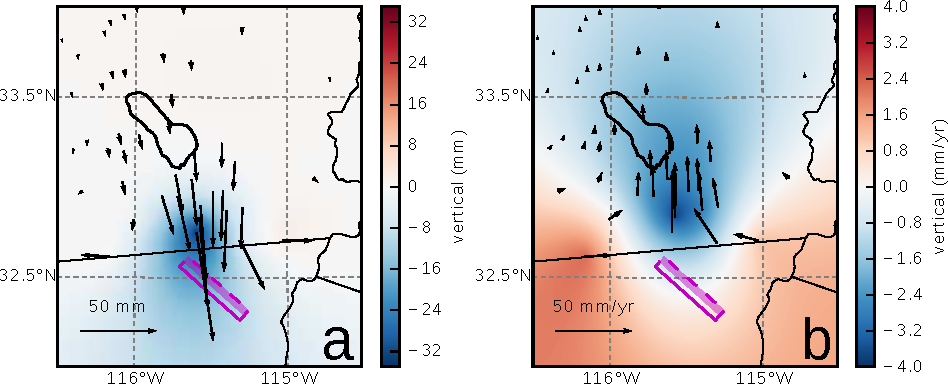
\includegraphics[scale=1.0]{ch3/figures/2016jb013114-p09}
\caption
[Postseismic displacements resulting from deep fault slip and a weak
lower crust]
{Displacements resulting from fault slip at lower crustal
depths (a), and initial velocities resulting from subsequent
relaxation of a viscoelastic lower crust (b).  The fault segment dips
$75^\circ$ to the north-east and its surface projection is outlined in
magenta.  The highlighted area on the fault extends from 15 to 30 km
depth and indicates where 1 meter of right-lateral slip was imposed.
The elastic properties of the crust and mantle are the same as in
Table 4.1, and $\eta_\mathrm{eff}$ is $10^{18}$ Pa s in the lower crust.
Vertical displacements are interpolated between station locations.}
\label{ch3:fig:LowerCrust} 
\end{figure}
 
We must determine at which point the early postseismic approximation
breaks down, which we will denote as $t_{\mathrm{bd}}$.  As noted, eq.
(\ref{ApproxForward}) is valid for as long as the rate of deformation
resulting from viscoelastic relaxation is approximately constant. We
can almost certainly assume that deformation at the most far-field
stations, which are ${\sim}400$ km away from the El Mayor-Cucapah
epicenter, is the result of viscoelastic relaxation. The approximation
should then be valid for as long as a linear trend adequately
approximates the far-field deformation. Using this logic, it would
appear that $t_{\mathrm{bd}}$ is about one year after the El
Mayor-Cucapah earthquake.  Another way to determine $t_{\mathrm{bd}}$
is to find the best fitting prediction of eq. (\ref{ApproxForward}) to
observed deformation using increasing durations of the postseismic
time series.  $t_\mathrm{bd}$ should be the point when eq.
(\ref{ApproxForward}) is no longer capable of describing the observed
deformation without incurring systematic misfits.  When using eq.
(\ref{ApproxForward}) to fit the entire five years of postseismic
displacements, we see that the near-field displacements (e.g., station
P501) are accurately predicted. When looking at displacements in the
far-field (e.g., station P621), we see that eq. (\ref{ApproxForward})
overestimates the rate of deformation in the later postseismic period
and underestimates the rate of deformation in the early period (Figure
\ref{ch3:fig:RecordSection1}).  Due to the low signal-to-noise ratios
for far-field stations, it is difficult to determine at what point eq.
(\ref{ApproxForward}) is no longer able to predict the observed
displacements; however, we settle on $t_{\mathrm{bd}}=0.8$ years after
the earthquake, while acknowledging that the choice is subjective. As
noted in \citet{Hines2016}, overestimating $t_{\mathrm{bd}}$ will
result in a bias towards overestimating $\eta_{\mathrm{eff}}$, while
picking a $t_\mathrm{bd}$ which is too low will not necessarily result
in a biased estimate of $\eta_\mathrm{eff}$, although the
uncertainties would be larger. We can then consider inferences of
$\eta_{\mathrm{eff}}$ to be an upper bound on the viscosity needed to
describe the far-field rate of deformation during the first 0.8 years
of postseismic deformation.

\begin{figure}
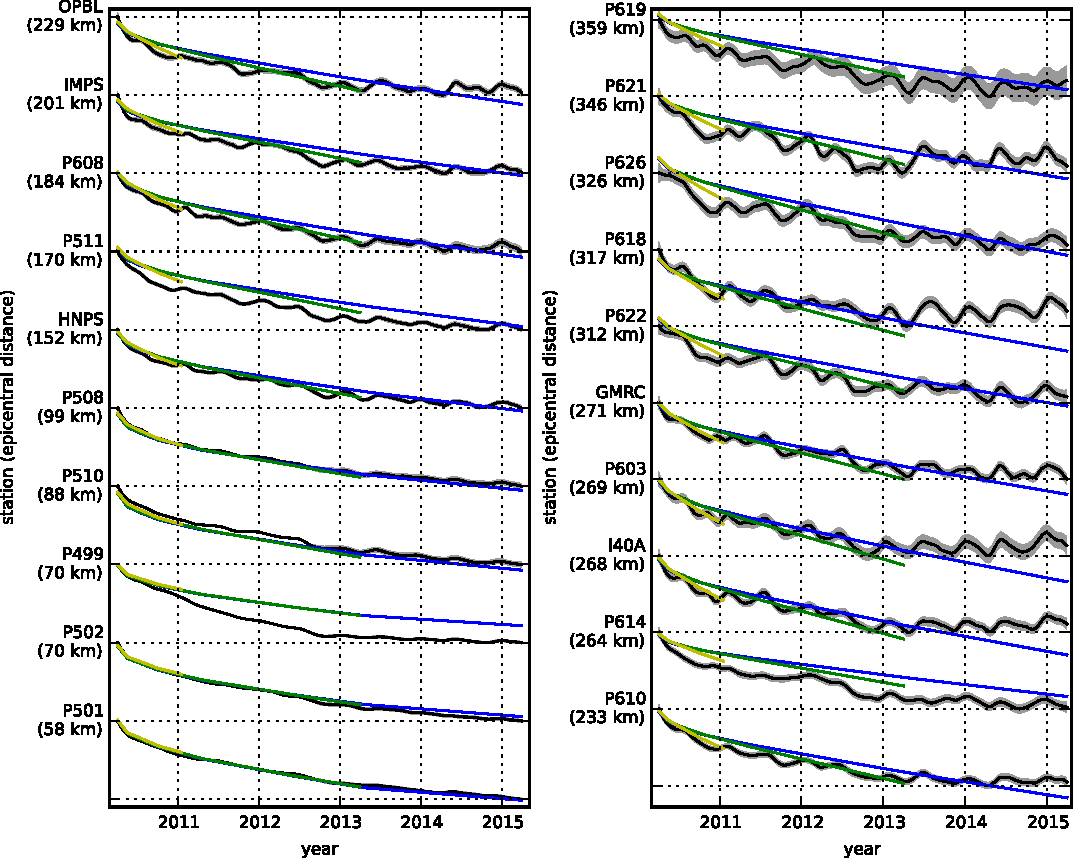
\includegraphics[scale=0.9]{ch3/figures/2016jb013114-p10}
\caption
[Observed postseismic displacments and predicted postseismic
displacments when using varying durations of the data]
{Observed postseismic displacements (black) and best fitting
predictions of eq. (\ref{ApproxForward}) to 5.0 (blue), 3.0 (green),
and 0.8 (yellow) years of the postseismic data.}
\label{ch3:fig:RecordSection1}
\end{figure}

We estimate coseismic slip, afterslip, and effective viscosities by
solving
\begin{equation}\label{ObjectiveFunction}
 \mathrm{min}_{s,\eta_\mathrm{eff}} \left(\left|\left|
 \frac{u_\mathrm{pred}(s,\eta_\mathrm{eff}) - u_\mathrm{post}}
 {\mathbf{\sigma_\mathrm{post}}}\right|\right|_2^2 + 
 \lambda_s||s||_2^2 + 
 \lambda_\eta||\nabla \eta_{\mathrm{eff}}^{-1}||_2^2\right),
\end{equation} 
where $u_\mathrm{post}$ consists of the first 0.8 years of postseismic
deformation and $u_\mathrm{pred}$ are the predicted displacements from
eq. (\ref{ApproxForward}).  Due to inherent non-uniqueness, we have
added zeroth-order Tikhonov regularization to estimates of $s$ and
second-order Tikhonov regularization to estimates of effective
fluidity $\eta_\mathrm{eff}^{-1}$. The degree to which we impose the
regularization on slip and fluidity is controlled by the penalty
parameters $\lambda_s$ and $\lambda_\eta$, which are chosen with
trade-off curves (Figure \ref{ch3:fig:S1}).  Our goal is to get a prior constraint
on $\eta_{\mathrm{eff}}$ to minimize the amount of searching we have
to do when describing the postseismic deformation over the full five
years, which we do in Section \ref{ch3:sec:FullInversion}.  Estimates
of $s$ made here will not be used in Section
\ref{ch3:sec:FullInversion}, and so the motivation behind adding
regularization to $s$ is to ensure that the slip driving viscoelastic
relaxation in eq. (\ref{ApproxForward}) is sensible.

Our initial estimate for coseismic slip and cumulative afterslip over
the first 0.8 years after the El Mayor-Cucapah earthquake are shown in
Figure \ref{ch3:fig:InitialSlip}.  Similar to our elastic slip model
from Section \ref{ch3:sec:ElasticInversion}, a significant amount of
right-lateral and normal coseismic slip is inferred to be on the
Sierra Cucapah segment. Our coseismic slip solution on the Sierra
Cucapah segment is consistent with field studies \citep{Fletcher2014}
and the model from \citet{Wei2011}.  Our inferred slip on the Indiviso
fault segment differs from \citet{Wei2011} because the GPS data used
in this study is not capable of resolving the spatial distribution of
fault slip on that segment (Figure \ref{ch3:fig:S2}).  The potency of inferred
coseismic slip is $3.3\times 10^{9}\ \mathrm{m}^3$, which is also
about the same as that inferred from Section
\ref{ch3:sec:ElasticInversion}. The present inference of afterslip on
the Indiviso fault is significantly less than what was found in the
Section \ref{ch3:sec:ElasticInversion} where we did not account for
viscoelasticity. When fault slip is simultaneously estimated with
viscosity, the potency of inferred afterslip over the first 0.8 years
after the earthquake is $0.85\times 10^9\ \mathrm{m}^3$, compared to
$3.5\times10^{9}\ \mathrm{m}^3$ when we assume the crust and upper
mantle are elastic.  The significant amount of afterslip inferred on
the Indiviso fault in Section \ref{ch3:sec:ElasticInversion} seems to
be compensating for unmodeled viscoelastic relaxation.  The fact that
there is still an appreciable amount of afterslip inferred on the
Indiviso fault raises the question of whether it is compensating for
viscoelastic relaxation that is more localized than what we allow for
since we only estimate depth dependent variations in viscosity.

Our estimated effective viscosities, and corresponding fluidities, are
shown in Figure \ref{ch3:fig:EffectiveViscosity}.  Although fluidity
is rarely used in geophysical literature, eq. (\ref{InitialRate}) is
linear with respect to fluidity and so the fluidity indicates the
amplitude of the viscoelastic signal coming from each layer.  We use
bootstrapping to find the 95\% confidence intervals for our estimated
effective viscosities which are shown as shaded regions in Figure
\ref{ch3:fig:EffectiveViscosity}.  It is important to remember that
the presented effective viscosities were estimated with a smoothing
regularization constraint and so the uncertainties are almost
certainly underestimated \citep{Aster2011}.  Indeed, many viscosity
profiles which are outside of the shown confidence intervals can just
as adequately described the first 0.8 years of postseismic
deformation. Our solution in Figure \ref{ch3:fig:EffectiveViscosity}
should be interpreted as the smoothest effective viscosity profile
which is capable of describing the data.  This means that any sharp
viscosity transitions will be tapered out in the inversion, which we
demonstrate with a synthetic test in Figure \ref{ch3:fig:S2}.  Nonetheless, a robust
feature that we see with a variety of choices for $\lambda_s$,
$\lambda_\eta$, and $t_\mathrm{bd}$ is that the largest jump in
fluidity is at 60 km depth, which is consistent with the range of
lithosphere-asthenosphere boundary depths inferred by
\citet{Lekic2011}. This transitional depth is also consistent with the
the viscosity structure required to explain far-field postseismic
deformation following the Hector Mine earthquake \citep{Freed2007a}.
We find that the viscosity below 60 km depth needs to be
${\sim}1\times10^{18}$ Pa s to describe the early rate of postseismic
deformation at far-field stations while the lower crust and uppermost
mantle need to be relatively stronger.  The viscosity of the lower
crust has the largest uncertainties because there is no evidence of
relaxation in that layer, meaning that it is effectively elastic over
the first 0.8 years after the earthquake.

\begin{figure}
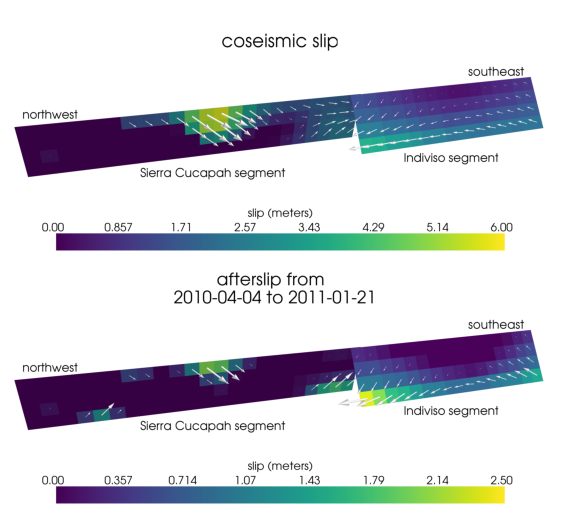
\includegraphics[scale=1.0]{ch3/figures/2016jb013114-p11}
\caption
[Coseismic slip and afterslip inferred from 0.8 years of postseismic
data]
{Coseismic slip and afterslip inferred by fitting eq.
(\ref{ApproxForward}) to the first 0.8 years of postseismic
displacements.}
\label{ch3:fig:InitialSlip}
\end{figure} 

\begin{figure}
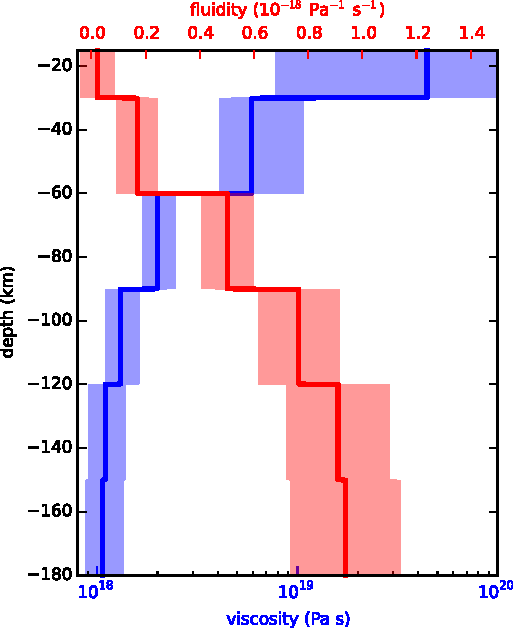
\includegraphics[scale=1.0]{ch3/figures/2016jb013114-p12}
\caption
[Inferred effective viscosities]
{Effective viscosities and associated fluidities inferred by
fitting eq. (\ref{ApproxForward}) to the first 0.8 years of
postseismic displacements. 95\% confidence intervals, estimated from
bootstrapping, are indicated by shaded regions.}
\label{ch3:fig:EffectiveViscosity}
\end{figure} 

\subsection{Full postseismic inversion}\label{ch3:sec:FullInversion} 
In the previous section, we used the inverse method from
\citet{Hines2016} to constrain the effective viscosity structure
required to explain the first 0.8 years of postseismic deformation. In
this section, we use these effective viscosities as a prior constraint
when searching for models which are capable of describing the
available five years of postseismic data, where our forward problem is
now eq. (\ref{GeneralForward}) rather than the approximation given by
eq. (\ref{ApproxForward}).  We perform a series of fault slip
inversions assuming a variety of rheologies for the lower crust and
upper mantle which are consistent with our findings from Section
\ref{ch3:sec:InitialInversion}.  We appraise each model using the mean
chi-squared value,
\begin{equation}\label{ch3:eq:Misfit}
  \bar\chi^2 = \frac{1}{N}\left|\left|\frac{u_\mathrm{pred} - u_\mathrm{post}}{\sigma_\mathrm{post}}\right|\right|_2^2,
\end{equation}
where $N$ is the number of observations.

We first assume that the crust and mantle can be described with a
Maxwell rheology, and we set the steady-state viscosity,
$\eta_\mathrm{M}$, equal to our inference of $\eta_{\mathrm{eff}}$.
We compute $f$ and $g$ from eq. (\ref{GeneralForward}) using Pylith,
and we use the same spatial and temporal discretization of $s$ as in
Sections \ref{ch3:sec:ElasticInversion} and
\ref{ch3:sec:InitialInversion}. We estimate $s$ using linear least
squares and find a misfit of $\bar\chi^2=37.4$. For comparison,
$\bar\chi^2=35.3$ for the elastic model from Section
\ref{ch3:sec:ElasticInversion}.  The Maxwell viscoelastic model has a
larger misfit because it tends to overestimate the rate of deformation
after about three years (Figure \ref{ch3:fig:RecordSectionMain}).
Since our initial estimates of $\eta_\mathrm{eff}$ may be biased
towards overestimating viscosities, we have also performed the slip
inversion where we use uniformly lower viscosities in the crust and
mantle; however, decreasing the viscosity only increases the misfit.
Although, the viscosities used here are consistent with the successful
Maxwell viscoelastic models found by \citet{Rollins2015} and
\citet{Spinler2015}, which had mantle viscosities on the order of
$10^{18}$ Pa s and relatively higher lower crustal viscosities, we
find that such a model is incapable of describing the entire
postseismic time series.  \citet{Pollitz2001} similarly recognized
this deficiency in a Maxwell rheology, which then motivated their
exploration of a Burgers rheology upper mantle \citep{Pollitz2003}.

Instead of exploring a Burgers rheology mantle, which introduces two
new parameters that need to be estimated, the transient viscosity,
$\eta_{K}$, and transient shear modulus, $\mu_{K}$, we first consider
a Zener rheology for the mantle, which only introduces one unknown
model parameter, $\mu_{K}$.  We assume that the lower crust still has
a Maxwell rheology. The steady-state viscosity in the crust and the
transient viscosity in the mantle are set equal to the inferred
effective viscosities.  We then estimate the ratio of shear moduli,
$\frac{\mu_K}{\mu}$. We compute nine different sets of Green's
functions, $f$ and $g$, where we assume values of $\frac{\mu_K}{\mu}$
ranging from 0 to 1. The former being a degenerate case where the
Zener model reduces to the above Maxwell model.  We estimate coseismic
slip and afterslip for each realization of $\frac{\mu_K}{\mu}$.  We
find that a shear moduli ratio of 0.375 yields the best prediction to
the observed postseismic displacements with a misfit of
$\bar\chi^2=31.2$ (Figure \ref{ch3:fig:ShearModulusRatio}).  The
improvement in the Zener model over the Maxwell model can be seen in
the fit to the far-field data (Figure \ref{ch3:fig:RecordSectionMain})
where the Zener model does a significantly better job at explaining
the transient rate of deformation throughout the five years considered
in this study.  The rheologic parameters for our preferred Zener model
are summarized in Table 4.1.

\begin{figure}
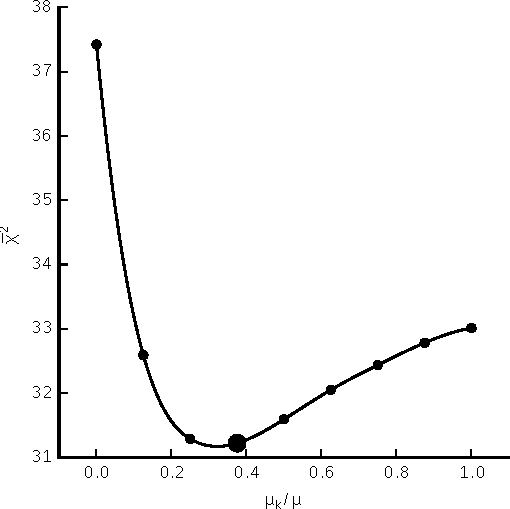
\includegraphics[scale=1.0]{ch3/figures/2016jb013114-f13}
\caption
[Misfit as a function of transient shear modulus]
{Mean chi-squared value as a function of the transient shear
modulus relative to the elastic shear modulus in a Zener rheology
upper mantle. Large dot indicates our preferred ratio.}
\label{ch3:fig:ShearModulusRatio}
\end{figure}

Because we are able to adequately describe the available five years of
postseismic deformation with a Zener model, we do not find it
necessary to explore the parameter space for a more complicated
Burgers rheology.  However, since the Zener model is a Burgers model
with an infinite steady-state viscosity, we can conclude that any
Burgers rheology that has a transient viscosity consistent with that
found in Section \ref{ch3:sec:InitialInversion} and a steady-state
viscosity $\gtrsim10^{20}$ Pa s, which is effectively infinite on the
time scale of five years, would also be able to satisfactorily
describe the observable postseismic deformation.
  
The regularized inference of coseismic slip and afterslip for our
preferred Zener model is shown in Figure \ref{ch3:fig:FinalSlip}.  The
inferred coseismic potency is $3.0\times10^{9}\ \mathrm{m}^3$,
equivalent to a Mw=7.26 earthquake, where most of the slip is shallow
and on the Sierra Cucapah fault segment.  The potency of five years of
afterslip is $1.1\times10^{9}\ \mathrm{m}^3$. Most of the afterslip in
our preferred model occurs within the first year after the earthquake
and coincides with the location of our inferred coseismic slip.
Inferred afterslip within the first year is accounting for the most
rapid near-field transient deformation (Figure \ref{ch3:fig:S3}).  After one year,
afterslip is inferred to be deeper down on the Sierra Cucapah segment.
The sustained near-field postseismic deformation is being explained by
this continued afterslip as well as viscoelastic relaxation in the
lower crust. We emphasize, that the GPS station closest to where we
infer afterslip, P496, is still about 30 km away, which is too far for
us to conclusively discern deep afterslip from viscoelastic relaxation
in the lower crust.  The deep afterslip inferred after one year could
potentially be compensating for an overestimated lower crustal
viscosity.  To test this, we have modified our preferred model by
decreasing the lower crustal viscosity from $4.4\times10^{19}$ Pa s
to $1\times10^{19}$ Pa s, which is still consistent with our viscosity
inference from Section \ref{ch3:sec:InitialInversion}, and we inverted
for fault slip.  We find that a model with a weaker lower crust
adequately describes the postseismic displacements without any
afterslip after one year, while still requiring about the same amount
of afterslip over the first year. We do believe that the early
afterslip on the Sierra Cucapah segment is a robust feature in our
preferred model, while we are not confident in our inference of later
deep afterslip.

The postseismic displacements predicted by our preferred Zener model
are shown in Figures \ref{ch3:fig:NearField}, \ref{ch3:fig:FarField}
and \ref{ch3:fig:RecordSectionMain}.  The largest misfit occur within
the Imperial Valley where there does not appear to be any systematic
trend in the residuals.  This suggests that the large errors are due
to localized processes such as fault slip in the Imperial Valley
triggered by the El Mayor-Cucapah earthquake \citep{Wei2011a,Wei2015}.
We do not see any pattern in the residuals that would suggest a
laterally heterogeneous viscosity structure, which has been explored
by \citet{Pollitz2012} and \citet{Rollins2015}.  We do notice regional
scale seasonal oscillations in the lateral and vertical components of
the residuals with an amplitude of 1-2 millimeters.  This is the
result of our method for data processing which is not able to
completely remove the seasonal signal in the GPS data, which was
discussed in Section \ref{ch3:sec:Data}.  Additionally, we see
systematic misfit in the later postseismic period west of the Landers
and Hector Mine earthquakes, which may be the result of unmodeled
postseismic deformation following those earthquakes.  Lastly, there
are clear discrepancies between the observed and predicted vertical
displacements following the first year after the El Mayor-Cucapah
earthquake. We observe a broad uplift throughout Southern California
which is inconsistent with any postseismic model.

\begin{figure}
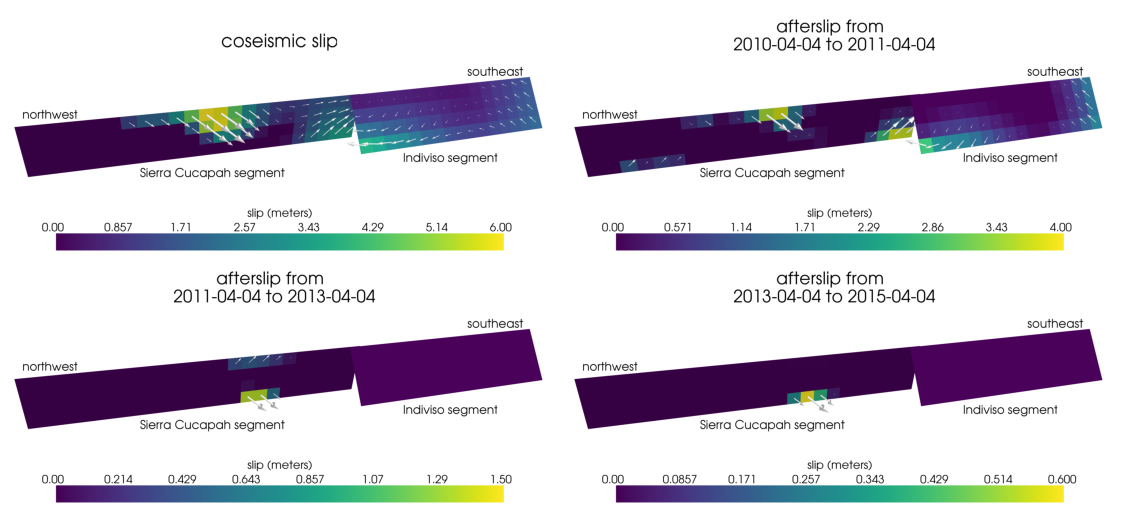
\includegraphics[scale=0.9]{ch3/figures/2016jb013114-p14}
\caption
[Coseismic slip and afterslip inferred from all available postseismic
data]
{Inferred coseismic slip and afterslip for our preferred
model, which has a Maxwell rheology in the lower crust and a Zener
rheology in the upper mantle.  The transient viscosity, $\eta_K$, in
the mantle and steady-state viscosity, $\eta_M$, in the crust are set
equal to the effective viscosities from Figure
\ref{ch3:fig:EffectiveViscosity}. We use $\frac{\mu_K}{\mu}=0.375$ in
the upper mantle.}
\label{ch3:fig:FinalSlip}
\end{figure}
  
\section{Discussion}\label{Discussion}
It has long been recognized that deep afterslip and viscoelastic
relaxation following an upper crustal earthquake can result in similar
horizontal ground deformation at the surface
\citep[e.g.,][]{Savage1990, Pollitz2001, Hearn2003, Feigl2006}. The
similarity of the horizontal postseismic deformation results in a
non-uniqueness in inferences of afterslip or viscoelastic relaxation.
The spatial pattern of vertical postseismic deformation has been
proposed to be a discriminant between deep afterslip and viscoelastic
relaxation \citep[e.g.,][]{Pollitz2001, Hearn2003}. It is, however,
important to note that patterns of vertical deformation are very
sensitive to the depth-dependence of viscosity below the upper crust
\citep{Yang1981,Hetland2014}.  The similarity between deformation
resulting from deep afterslip and viscoelastic relaxation of coseismic
stresses is different from the ill-posedness described in Section
\ref{ch3:sec:InitialInversion}. In our method, any inferred afterslip
will also mechanically drive additional viscoelastic relaxation.  The
horizontal deformation resulting from deep afterslip will generally be
in the opposite direction as horizontal deformation resulting from
viscoelastic relaxation of subsequent stresses in the lower crust
(Figure \ref{ch3:fig:LowerCrust}).  As a result, there is a trade-off
between inferences of deep afterslip and lower crustal viscosity.  In
our synthetic tests in \citet{Hines2016}, we have found that inverting
surface deformation for afterslip and viscosity within the same depth
interval tends to result in overestimated afterslip and an
underestimated viscosity.

Most postseismic studies assume Maxwell viscoelasticity in the lower
crust and upper mantle \citep[e.g.,][]{Nur1974, Pollitz2000,
Hetland2003, Freed2006a, Johnson2009, Hearn2009}, which is the
simplest viscoelastic rheologic model.  In Southern California,
postseismic studies following the Landers \citep{Pollitz2000}, Hector
Mine \citep{Pollitz2001}, and El Mayor-Cucapah earthquake
\citep{Spinler2015,Rollins2015}, have assumed Maxwell viscoelasticity
in the lower crust and upper mantle and have inferred upper mantle
viscosities on the order of $10^{17}$ to $10^{18}$ Pa s and lower
crust viscosities $\gtrsim 10^{19}$ Pa s. These postseismic studies
are consistent with \citet{Kaufmann2000} and \citet{Cavalie2007}, who
found that an upper mantle viscosity of $10^{18}$ Pa s and a crustal
viscosity $\gtrsim10^{20}$ Pa s are necessary to describe subsidence
resulting from changes in loading from Lake Mead. This isostatic
adjustment is a process with similar spatial and temporal scales as
postseismic deformation, and thus the inferred viscosities of these
two types of studies would likely agree. While these studies found
viscosities that are consistent with our effective viscosities from
Section \ref{ch3:sec:InitialInversion}, they are inconsistent with
viscosity estimates made from geophysical processes that occur over
longer time scales. For example, \citet{Lundgren2009} found that lower
crust and upper mantle viscosities on the order of $10^{21}$ and
$10^{19}$ Pa s, respectively, are needed to describe interseismic
deformation along the Southern San Andreas fault zone in the Salton
Sea region.  An even higher mantle viscosity, on the order of
$10^{20}$ Pa s, is required to describe isostatic adjustment resulting
from the draining of Lake Bonneville, which occurs on the time scales
of $10^{4}$ years \citep{Crittenden1967, Bills1987}.

An additional deficiency with the Maxwell rheology is that it predicts
a steady decay in the rate of postseismic deformation over time, which
fails to describe the commonly observed rapid, early transience
followed by a relatively steady rate of postseismic deformation.  One
could explain the early transient postseismic deformation with fault
creep and the later phase with relaxation in a Maxwell viscoelastic
lower crust and upper mantle \citep[e.g][]{Hearn2009,Johnson2009}.
However, postseismic deformation at distances greater than ${\sim}200$
km from the El Mayor-Cucapah epicenter can only be attributed to
viscoelastic relaxation \citep[e.g.,][]{Freed2007a} and we have
demonstrated that the far-field deformation cannot be explained with a
Maxwell rheology (Figure \ref{ch3:fig:RecordSectionMain}).

We found that a Zener rheology in the upper mantle with a transient
viscosity of ${\sim}10^{18}$ Pa s does a noticeably better job at
predicting far-field postseismic deformation.  A generalization of the
Zener viscoelastic model, schematically represented as several Kelvin
elements connected in series, is commonly used to describe seismic
attenuation \citep{Liu1976}.  The highest viscosity needed to describe
seismic attenuation is on the order of $10^{16}$ Pa s \citep{Yuen1982}
which has a characteristic relaxation time on the order of days. Even
though our inferred transient viscosity is orders of magnitude larger
than that required for seismic attenuation models, the two models are
not incompatible.  Rather, the delayed elasticity in seismic
attenuation models occurs on such short time scales that it can be
considered part of the instantaneous elastic phase of deformation
associated with the preferred Zener model in this study.

Of course, a Zener rheology provides an incomplete description of the
asthenosphere because it does not have the fluid-like behavior
required to explain isostatic rebound or convection in the mantle
\citep{OConnell1971}.  \citet{Yuen1982} proposed a Burgers rheology
with a low transient viscosity ($\eta_K\approx10^{16}$ Pa s) and high
steady-state viscosity ($\eta_M\approx10^{21}$ Pa s) to describe both
seismic attenuation and long term geologic processes.  The
justification of a Burger's rheology mantle is further supported by
laboratory experiments on olivine \citep{Chopra1997}.
\citet{Pollitz2003} sought to describe postseismic deformation
following Hector Mine with a Burgers rheology mantle and they found a
best fitting transient viscosity of $1.6\times10^{17}$ Pa s and
steady-state viscosity of $4.6\times10^{18}$ Pa s. While the Burgers
rheology was introduced as a means of bridging the gap between
relaxation observed in long and short term geophysical processes, the
inferred steady state viscosity from \citet{Pollitz2003} is still
inconsistent with the Maxwell viscosities inferred from studies on the
earthquake cycle and Lake Bonneville.  The transient viscosity
inferred by \citet{Pollitz2003} is constrained by the earliest phase
of postseismic deformation following the Hector Mine earthquake. While
\citet{Pollitz2003} ruled out deep afterslip as an alternative
mechanism based on inconsistent vertical deformation, it is still
possible to successfully describe all components of early postseismic
deformation following the Hector Mine earthquake with afterslip at
seismogenic depths \citep{Jacobs2002}. It is then possible that the
preferred rheologic model from \citet{Pollitz2003} was biased towards
inferring a particularly low transient viscosity by neglecting to
account for afterslip.  This is in contrast to the present study,
where we have inferred a viscosity structure simultaneously with
afterslip.  We also argue that a transient rheology is necessary to
explain postseismic deformation; however, our preferred transient
viscosity of ${\sim}10^{18}$ Pa s in the upper mantle is an order of
magnitude larger than the transient viscosity found by
\citet{Pollitz2003}.  The transient viscosity inferred here is
consistent with the results of \citet{Pollitz2015}, who reanalyzed
postseismic data following the Landers and Hector Mine earthquake
allowing the first few months of transient deformation to be described
by afterslip.  Since a Zener model is able to describe the available
postseismic deformation following the El Mayor-Cucapah earthquake, any
Burgers rheology with a steady-state viscosity that is
$\gtrsim10^{20}$ Pa s, effectively infinite over five years, would
also be able to describe the postseismic deformation. Such a Burgers
model might then be consistent with the steady-state viscosities
necessary for lake loading, interseismic deformation, and mantle
dynamics.

\section{Conclusion}
We have extracted a smoothed estimate of postseismic deformation
following the El Mayor-Cucapah earthquake from GPS displacement time
series.  Our estimated postseismic deformation reveals far-field
(epicentral distances ${\gtrsim}200$ km) transient deformation which
is undetectable after about three years. Near-field deformation
exhibits transience that decays to a sustained, elevated rate after
about one or two years.  We found that near-field transient
deformation can be explained with shallow afterslip.  The sustained
rate of near-field deformation can be explained with viscoelastic
relaxation in the lower crust and possibly continued afterslip.
Far-field transient deformation can be more definitively ascribed to
viscoelastic relaxation at depths greater than ${\sim}60$ km. Beneath
that depth, a transient viscosity of ${\sim}1\times10^{18}$ Pa s is
required to describe the rate of far-field deformation throughout the
five years considered in this study.  By describing the available
postseismic deformation with a transient rheology in the mantle, our
preferred model does not conflict with the generally higher
steady-state viscosities inferred from geophysical processes occurring
over longer time scales.

\section{Acknowledgements}
We thank Andy Freed for an illuminating discussion on the data used in
this study.  We thank Fred Pollitz and an anonymous reviewer for
comments that improved this manuscript. We also thank the editor,
Martha Savage.  This material is based on EarthScope Plate Boundary
Observatory data services provided by UNAVCO through the GAGE Facility
with support from the National Science Foundation (NSF) and National
Aeronautics and Space Administration (NASA) under NSF Cooperative
Agreement No. EAR-1261833.  The data used in this study can be found
at www.unavco.org. This material is based upon work supported by the
National Science Foundation under Grant Numbers EAR 1045372 and EAR
1245263.

%\bibliographystyle{agu04}
%\bibliography{refs}

\section{Supporting information}
Figures \ref{ch3:fig:S1} and \ref{ch3:fig:S2} provide additional
information about the inversion in Section \ref{ch3:sec:Model} of the
main text. Figures \ref{ch3:fig:S3} and \ref{ch3:fig:S4} show the
predicted displacements, which have been decomposed into elastic and
viscoelastic components, for the preferred model from Section
\ref{ch3:sec:FullInversion}.

\begin{figure}
\noindent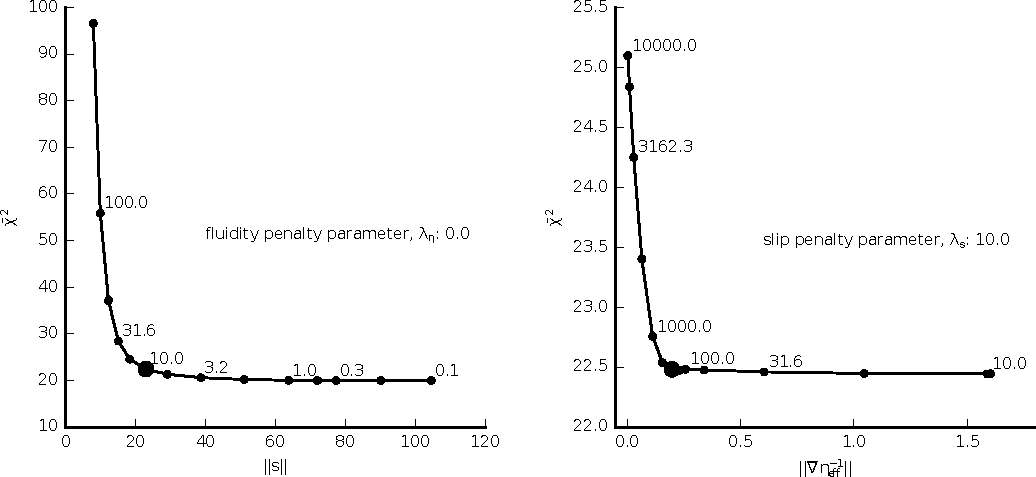
\includegraphics[scale=0.9]{ch3/figures/2016jb013114-fS01}
\caption
[Trade-off curves]
{Trade-off curves used to determine the damping parameters
$\lambda_s$ and $\lambda_\eta$ in eq.  (15) of the main text.  The
left panel shows the trade-off curve for the fault slip penalty
parameter, $\lambda_s$.  We pick $\lambda_s$ while keeping the penalty
parameter for fluidity, $\lambda_\eta$, fixed at zero.  The right
panel shows the trade of curve for selecting $\lambda_\eta$, where we
fix $\lambda_s$ at the chosen value from the left panel. Chosen values
are indicated with the larger marker.  When picking $\lambda_s$, we
try to find a good balance between the mean chi-squared value,
$\bar{\chi}^2$, and the size of the slip parameters, $||s||$.  Our
choice of $\lambda_\eta$ is a balance between $\bar{\chi}^2$ and the
size of the Laplacian of fluidity, $||\nabla
\eta_\mathrm{eff}^{-1}||$.}
\label{ch3:fig:S1}
\end{figure}

\begin{figure}
\noindent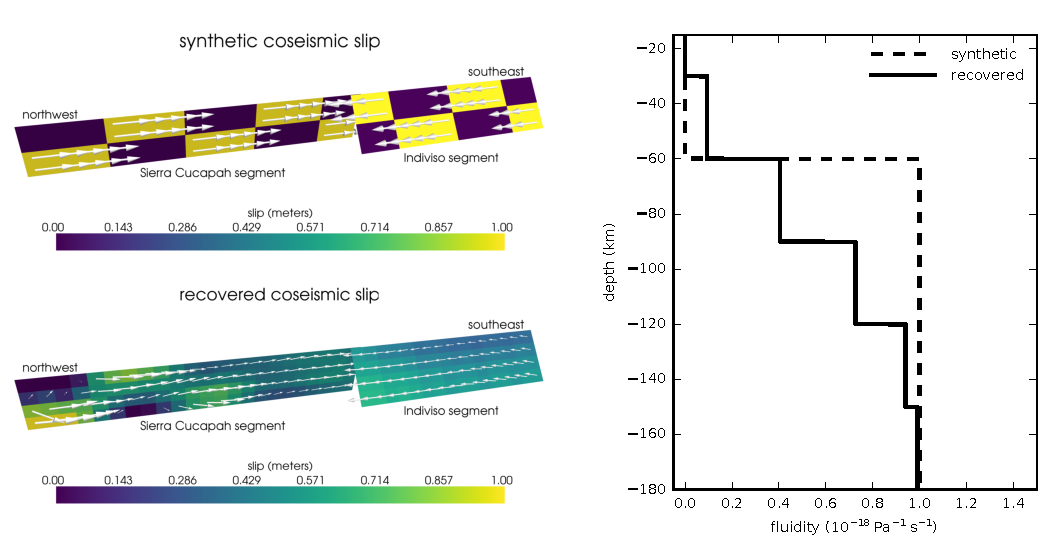
\includegraphics[scale=0.9]{ch3/figures/2016jb013114-pS02}
\caption
[Synthetic checkerboard test]
{Checkerboard test used to assess the resolving power of the
inversion in Section \ref{ch3:sec:InitialInversion} of the main text.  We create synthetic data
at all of the GPS stations considered in this study by evaluating eq.
(14) with the synthetic coseismic slip distribution and fluidity
distributions. Our synthetic fluidity model has a jump from 0.0 to
$10^{-18}$ Pa$^{-1}$ s$^{-1}$ at 60 km depth.  Our synthetic slip
model does not include afterslip, although we estimate afterslip along
with coseismic slip and fluidity in this test.  We estimate these
values in the same way as described in the main text and we also use
the same penalty parameters.  We do not add any noise to our synthetic
data so that the recovered model just indicates how much the
regularization influences the solution.  Note that our ability to
recover slip decreases towards the southern end of the fault, farthest
from the available data.  Also note that the smoothing constraint on
fluidity largely obscures the jump in the synthetic model.}
\label{ch3:fig:S2}
\end{figure}

\begin{figure}
\noindent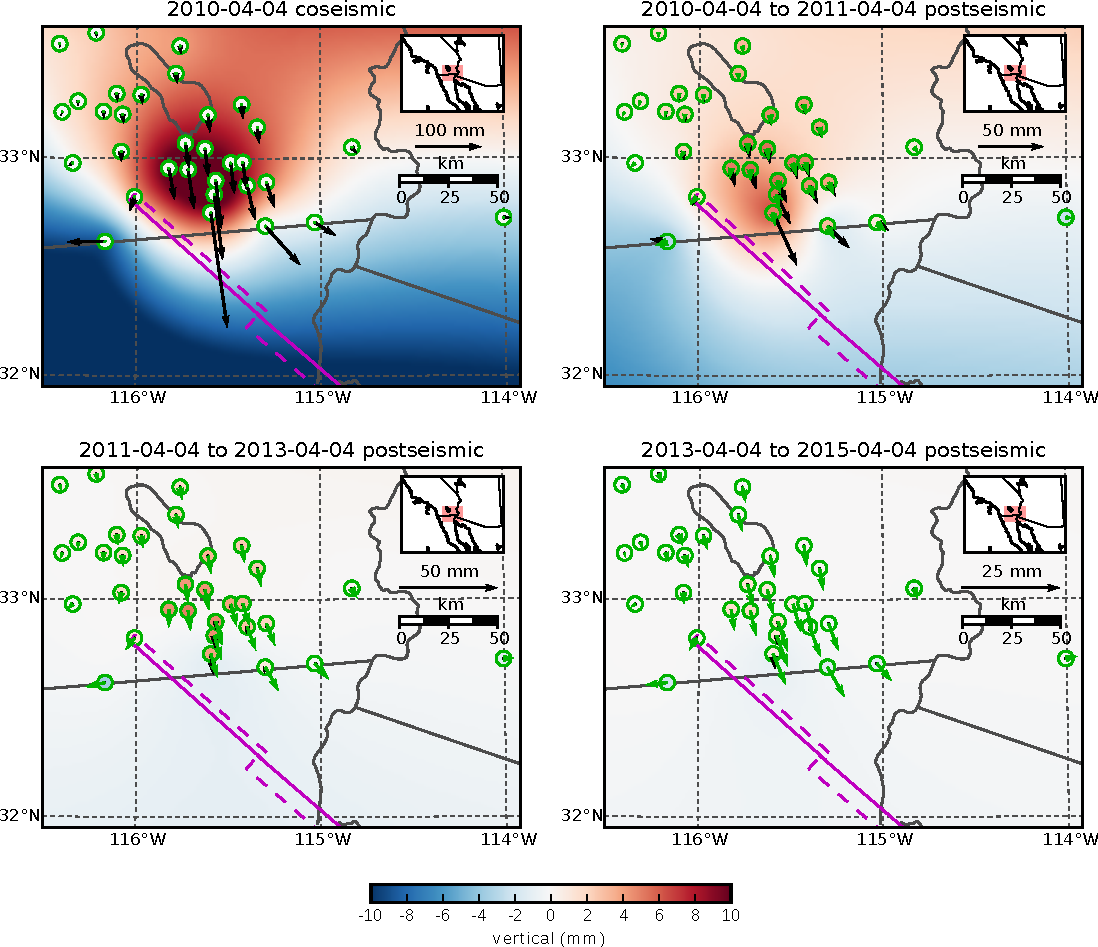
\includegraphics[scale=0.9]{ch3/figures/2016jb013114-pS03}
\caption
[Elastic and viscous components of predicted near-field postseismic
displacments]
{Elastic (black) and viscoelastic (green) components of the near-field
predicted displacements for the preferred Zener model from Section
\ref{ch3:sec:FullInversion}.  The elastic component is the deformation
resulting from fault slip and the viscoelastic component is the
deformation resulting from viscoelastic relaxation of stresses induced
by the fault slip. The elastic and viscoelastic components are
calculated from the first and second terms in eq.
(\ref{GeneralForward}), respectively.  The vertical elastic
component is shown as an interpolated field and the vertical
viscoelastic component is shown within the green circles.}
\label{ch3:fig:S3}
\end{figure}

\begin{figure}
\noindent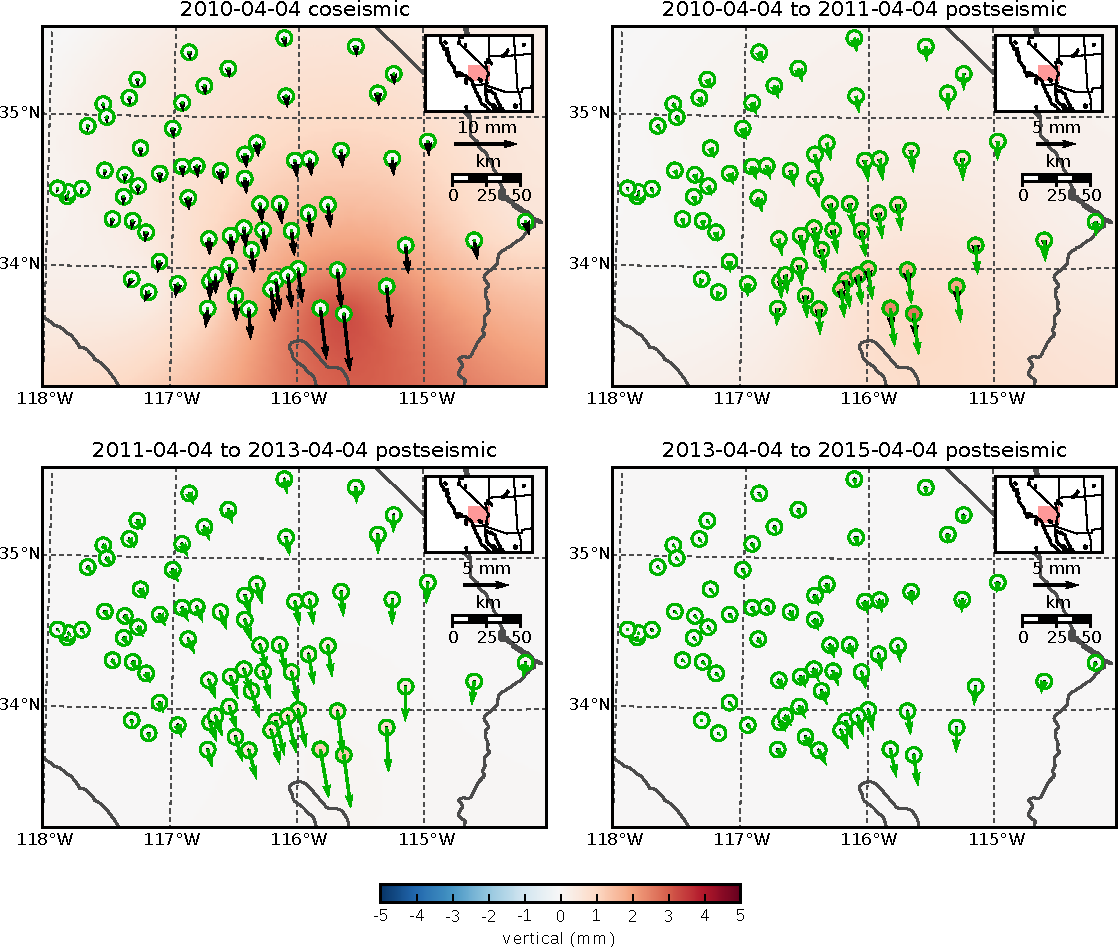
\includegraphics[scale=0.9]{ch3/figures/2016jb013114-pS04}
\caption
[Elastic and viscous components of predicted far-field postseismic
displacments]
{Same as figure \ref{ch3:fig:S3} but for far-field stations.}
\label{ch3:fig:S4}
\end{figure}

